\documentclass{report}

\usepackage[T2A]{fontenc}
\usepackage[russian]{babel}
\usepackage{graphicx}
\usepackage{float}
\usepackage{hyperref}
\usepackage{amsmath}
\usepackage{diffcoeff,amssymb}
\usepackage{mathtools}
\usepackage[normalem]{ulem}
\usepackage{physics}
\usepackage{wrapfig}
\usepackage{float} % для позиционирования [H]
\usepackage{siunitx} % для градусов и единиц измерения

%%%%%%%%%%%%%%%%%%%%%%%%%%%%%%%%%
% PACKAGE IMPORTS
%%%%%%%%%%%%%%%%%%%%%%%%%%%%%%%%%


\usepackage[tmargin=2cm,rmargin=1in,lmargin=1in,margin=0.85in,bmargin=2cm,footskip=.2in]{geometry}
\usepackage{amsmath,amsfonts,amsthm,amssymb,mathtools}
\usepackage[varbb]{newpxmath}
\usepackage{xfrac}
\usepackage[makeroom]{cancel}
\usepackage{mathtools}
\usepackage{bookmark}
\usepackage{enumitem}
\usepackage{hyperref,theoremref}
\hypersetup{
	pdftitle={Assignment},
	colorlinks=true, linkcolor=doc!90,
	bookmarksnumbered=true,
	bookmarksopen=true
}
\usepackage[most,many,breakable]{tcolorbox}
\usepackage{xcolor}
\usepackage{varwidth}
\usepackage{varwidth}
\usepackage{etoolbox}
%\usepackage{authblk}
\usepackage{nameref}
\usepackage{multicol,array}
\usepackage{tikz-cd}
\usepackage[ruled,vlined,linesnumbered]{algorithm2e}
\usepackage{comment} % enables the use of multi-line comments (\ifx \fi) 
\usepackage{import}
\usepackage{xifthen}
\usepackage{pdfpages}
\usepackage{transparent}

\newcommand\mycommfont[1]{\footnotesize\ttfamily\textcolor{blue}{#1}}
\SetCommentSty{mycommfont}
\newcommand{\incfig}[1]{%
    \def\svgwidth{\columnwidth}
    \import{./figures/}{#1.pdf_tex}
}

\usepackage{tikzsymbols}
\renewcommand\qedsymbol{$\Laughey$}


%\usepackage{import}
%\usepackage{xifthen}
%\usepackage{pdfpages}
%\usepackage{transparent}


%%%%%%%%%%%%%%%%%%%%%%%%%%%%%%
% SELF MADE COLORS
%%%%%%%%%%%%%%%%%%%%%%%%%%%%%%



\definecolor{myg}{RGB}{56, 140, 70}
\definecolor{myb}{RGB}{45, 111, 177}
\definecolor{myr}{RGB}{199, 68, 64}
\definecolor{mytheorembg}{HTML}{F2F2F9}
\definecolor{mytheoremfr}{HTML}{00007B}
\definecolor{mylenmabg}{HTML}{FFFAF8}
\definecolor{mylenmafr}{HTML}{983b0f}
\definecolor{mypropbg}{HTML}{f2fbfc}
\definecolor{mypropfr}{HTML}{191971}
\definecolor{myexamplebg}{HTML}{F2FBF8}
\definecolor{myexamplefr}{HTML}{88D6D1}
\definecolor{myexampleti}{HTML}{2A7F7F}
\definecolor{mydefinitbg}{HTML}{E5E5FF}
\definecolor{mydefinitfr}{HTML}{3F3FA3}
\definecolor{notesgreen}{RGB}{0,162,0}
\definecolor{myp}{RGB}{197, 92, 212}
\definecolor{mygr}{HTML}{2C3338}
\definecolor{myred}{RGB}{127,0,0}
\definecolor{myyellow}{RGB}{169,121,69}
\definecolor{myexercisebg}{HTML}{F2FBF8}
\definecolor{myexercisefg}{HTML}{88D6D1}


%%%%%%%%%%%%%%%%%%%%%%%%%%%%
% TCOLORBOX SETUPS
%%%%%%%%%%%%%%%%%%%%%%%%%%%%

\setlength{\parindent}{1cm}
%================================
% THEOREM BOX
%================================

\tcbuselibrary{theorems,skins,hooks}
\newtcbtheorem[number within=section]{Theorem}{Theorem}
{%
	enhanced,
	breakable,
	colback = mytheorembg,
	frame hidden,
	boxrule = 0sp,
	borderline west = {2pt}{0pt}{mytheoremfr},
	sharp corners,
	detach title,
	before upper = \tcbtitle\par\smallskip,
	coltitle = mytheoremfr,
	fonttitle = \bfseries\sffamily,
	description font = \mdseries,
	separator sign none,
	segmentation style={solid, mytheoremfr},
}
{th}

\tcbuselibrary{theorems,skins,hooks}
\newtcbtheorem[number within=chapter]{theorem}{Theorem}
{%
	enhanced,
	breakable,
	colback = mytheorembg,
	frame hidden,
	boxrule = 0sp,
	borderline west = {2pt}{0pt}{mytheoremfr},
	sharp corners,
	detach title,
	before upper = \tcbtitle\par\smallskip,
	coltitle = mytheoremfr,
	fonttitle = \bfseries\sffamily,
	description font = \mdseries,
	separator sign none,
	segmentation style={solid, mytheoremfr},
}
{th}


\tcbuselibrary{theorems,skins,hooks}
\newtcolorbox{Theoremcon}
{%
	enhanced
	,breakable
	,colback = mytheorembg
	,frame hidden
	,boxrule = 0sp
	,borderline west = {2pt}{0pt}{mytheoremfr}
	,sharp corners
	,description font = \mdseries
	,separator sign none
}

%================================
% Corollery
%================================
\tcbuselibrary{theorems,skins,hooks}
\newtcbtheorem[number within=section]{Corollary}{Corollary}
{%
	enhanced
	,breakable
	,colback = myp!10
	,frame hidden
	,boxrule = 0sp
	,borderline west = {2pt}{0pt}{myp!85!black}
	,sharp corners
	,detach title
	,before upper = \tcbtitle\par\smallskip
	,coltitle = myp!85!black
	,fonttitle = \bfseries\sffamily
	,description font = \mdseries
	,separator sign none
	,segmentation style={solid, myp!85!black}
}
{th}
\tcbuselibrary{theorems,skins,hooks}
\newtcbtheorem[number within=chapter]{corollary}{Corollary}
{%
	enhanced
	,breakable
	,colback = myp!10
	,frame hidden
	,boxrule = 0sp
	,borderline west = {2pt}{0pt}{myp!85!black}
	,sharp corners
	,detach title
	,before upper = \tcbtitle\par\smallskip
	,coltitle = myp!85!black
	,fonttitle = \bfseries\sffamily
	,description font = \mdseries
	,separator sign none
	,segmentation style={solid, myp!85!black}
}
{th}


%================================
% LENMA
%================================

\tcbuselibrary{theorems,skins,hooks}
\newtcbtheorem[number within=section]{Lenma}{Lenma}
{%
	enhanced,
	breakable,
	colback = mylenmabg,
	frame hidden,
	boxrule = 0sp,
	borderline west = {2pt}{0pt}{mylenmafr},
	sharp corners,
	detach title,
	before upper = \tcbtitle\par\smallskip,
	coltitle = mylenmafr,
	fonttitle = \bfseries\sffamily,
	description font = \mdseries,
	separator sign none,
	segmentation style={solid, mylenmafr},
}
{th}

\tcbuselibrary{theorems,skins,hooks}
\newtcbtheorem[number within=chapter]{lenma}{Lenma}
{%
	enhanced,
	breakable,
	colback = mylenmabg,
	frame hidden,
	boxrule = 0sp,
	borderline west = {2pt}{0pt}{mylenmafr},
	sharp corners,
	detach title,
	before upper = \tcbtitle\par\smallskip,
	coltitle = mylenmafr,
	fonttitle = \bfseries\sffamily,
	description font = \mdseries,
	separator sign none,
	segmentation style={solid, mylenmafr},
}
{th}


%================================
% PROPOSITION
%================================

\tcbuselibrary{theorems,skins,hooks}
\newtcbtheorem[number within=section]{Prop}{Proposition}
{%
	enhanced,
	breakable,
	colback = mypropbg,
	frame hidden,
	boxrule = 0sp,
	borderline west = {2pt}{0pt}{mypropfr},
	sharp corners,
	detach title,
	before upper = \tcbtitle\par\smallskip,
	coltitle = mypropfr,
	fonttitle = \bfseries\sffamily,
	description font = \mdseries,
	separator sign none,
	segmentation style={solid, mypropfr},
}
{th}

\tcbuselibrary{theorems,skins,hooks}
\newtcbtheorem[number within=chapter]{prop}{Proposition}
{%
	enhanced,
	breakable,
	colback = mypropbg,
	frame hidden,
	boxrule = 0sp,
	borderline west = {2pt}{0pt}{mypropfr},
	sharp corners,
	detach title,
	before upper = \tcbtitle\par\smallskip,
	coltitle = mypropfr,
	fonttitle = \bfseries\sffamily,
	description font = \mdseries,
	separator sign none,
	segmentation style={solid, mypropfr},
}
{th}


%================================
% CLAIM
%================================

\tcbuselibrary{theorems,skins,hooks}
\newtcbtheorem[number within=section]{claim}{Claim}
{%
	enhanced
	,breakable
	,colback = myg!10
	,frame hidden
	,boxrule = 0sp
	,borderline west = {2pt}{0pt}{myg}
	,sharp corners
	,detach title
	,before upper = \tcbtitle\par\smallskip
	,coltitle = myg!85!black
	,fonttitle = \bfseries\sffamily
	,description font = \mdseries
	,separator sign none
	,segmentation style={solid, myg!85!black}
}
{th}



%================================
% Exercise
%================================

\tcbuselibrary{theorems,skins,hooks}
\newtcbtheorem[number within=section]{Exercise}{Exercise}
{%
	enhanced,
	breakable,
	colback = myexercisebg,
	frame hidden,
	boxrule = 0sp,
	borderline west = {2pt}{0pt}{myexercisefg},
	sharp corners,
	detach title,
	before upper = \tcbtitle\par\smallskip,
	coltitle = myexercisefg,
	fonttitle = \bfseries\sffamily,
	description font = \mdseries,
	separator sign none,
	segmentation style={solid, myexercisefg},
}
{th}

\tcbuselibrary{theorems,skins,hooks}
\newtcbtheorem[number within=chapter]{exercise}{Exercise}
{%
	enhanced,
	breakable,
	colback = myexercisebg,
	frame hidden,
	boxrule = 0sp,
	borderline west = {2pt}{0pt}{myexercisefg},
	sharp corners,
	detach title,
	before upper = \tcbtitle\par\smallskip,
	coltitle = myexercisefg,
	fonttitle = \bfseries\sffamily,
	description font = \mdseries,
	separator sign none,
	segmentation style={solid, myexercisefg},
}
{th}

%================================
% EXAMPLE BOX
%================================

\newtcbtheorem[number within=section]{Example}{Example}
{%
	colback = myexamplebg
	,breakable
	,colframe = myexamplefr
	,coltitle = myexampleti
	,boxrule = 1pt
	,sharp corners
	,detach title
	,before upper=\tcbtitle\par\smallskip
	,fonttitle = \bfseries
	,description font = \mdseries
	,separator sign none
	,description delimiters parenthesis
}
{ex}

\newtcbtheorem[number within=chapter]{example}{Example}
{%
	colback = myexamplebg
	,breakable
	,colframe = myexamplefr
	,coltitle = myexampleti
	,boxrule = 1pt
	,sharp corners
	,detach title
	,before upper=\tcbtitle\par\smallskip
	,fonttitle = \bfseries
	,description font = \mdseries
	,separator sign none
	,description delimiters parenthesis
}
{ex}

%================================
% DEFINITION BOX
%================================

\newtcbtheorem[number within=section]{Definition}{Definition}{enhanced,
	before skip=2mm,after skip=2mm, colback=red!5,colframe=red!80!black,boxrule=0.5mm,
	attach boxed title to top left={xshift=1cm,yshift*=1mm-\tcboxedtitleheight}, varwidth boxed title*=-3cm,
	boxed title style={frame code={
					\path[fill=tcbcolback]
					([yshift=-1mm,xshift=-1mm]frame.north west)
					arc[start angle=0,end angle=180,radius=1mm]
					([yshift=-1mm,xshift=1mm]frame.north east)
					arc[start angle=180,end angle=0,radius=1mm];
					\path[left color=tcbcolback!60!black,right color=tcbcolback!60!black,
						middle color=tcbcolback!80!black]
					([xshift=-2mm]frame.north west) -- ([xshift=2mm]frame.north east)
					[rounded corners=1mm]-- ([xshift=1mm,yshift=-1mm]frame.north east)
					-- (frame.south east) -- (frame.south west)
					-- ([xshift=-1mm,yshift=-1mm]frame.north west)
					[sharp corners]-- cycle;
				},interior engine=empty,
		},
	fonttitle=\bfseries,
	title={#2},#1}{def}
\newtcbtheorem[number within=chapter]{definition}{Definition}{enhanced,
	before skip=2mm,after skip=2mm, colback=red!5,colframe=red!80!black,boxrule=0.5mm,
	attach boxed title to top left={xshift=1cm,yshift*=1mm-\tcboxedtitleheight}, varwidth boxed title*=-3cm,
	boxed title style={frame code={
					\path[fill=tcbcolback]
					([yshift=-1mm,xshift=-1mm]frame.north west)
					arc[start angle=0,end angle=180,radius=1mm]
					([yshift=-1mm,xshift=1mm]frame.north east)
					arc[start angle=180,end angle=0,radius=1mm];
					\path[left color=tcbcolback!60!black,right color=tcbcolback!60!black,
						middle color=tcbcolback!80!black]
					([xshift=-2mm]frame.north west) -- ([xshift=2mm]frame.north east)
					[rounded corners=1mm]-- ([xshift=1mm,yshift=-1mm]frame.north east)
					-- (frame.south east) -- (frame.south west)
					-- ([xshift=-1mm,yshift=-1mm]frame.north west)
					[sharp corners]-- cycle;
				},interior engine=empty,
		},
	fonttitle=\bfseries,
	title={#2},#1}{def}



%================================
% Solution BOX
%================================

\makeatletter
\newtcbtheorem{question}{Question}{enhanced,
	breakable,
	colback=white,
	colframe=myb!80!black,
	attach boxed title to top left={yshift*=-\tcboxedtitleheight},
	fonttitle=\bfseries,
	title={#2},
	boxed title size=title,
	boxed title style={%
			sharp corners,
			rounded corners=northwest,
			colback=tcbcolframe,
			boxrule=0pt,
		},
	underlay boxed title={%
			\path[fill=tcbcolframe] (title.south west)--(title.south east)
			to[out=0, in=180] ([xshift=5mm]title.east)--
			(title.center-|frame.east)
			[rounded corners=\kvtcb@arc] |-
			(frame.north) -| cycle;
		},
	#1
}{def}
\makeatother

%================================
% SOLUTION BOX
%================================

\makeatletter
\newtcolorbox{solution}{enhanced,
	breakable,
	colback=white,
	colframe=myg!80!black,
	attach boxed title to top left={yshift*=-\tcboxedtitleheight},
	title=Solution,
	boxed title size=title,
	boxed title style={%
			sharp corners,
			rounded corners=northwest,
			colback=tcbcolframe,
			boxrule=0pt,
		},
	underlay boxed title={%
			\path[fill=tcbcolframe] (title.south west)--(title.south east)
			to[out=0, in=180] ([xshift=5mm]title.east)--
			(title.center-|frame.east)
			[rounded corners=\kvtcb@arc] |-
			(frame.north) -| cycle;
		},
}
\makeatother

%================================
% Question BOX
%================================

\makeatletter
\newtcbtheorem{qstion}{Question}{enhanced,
	breakable,
	colback=white,
	colframe=mygr,
	attach boxed title to top left={yshift*=-\tcboxedtitleheight},
	fonttitle=\bfseries,
	title={#2},
	boxed title size=title,
	boxed title style={%
			sharp corners,
			rounded corners=northwest,
			colback=tcbcolframe,
			boxrule=0pt,
		},
	underlay boxed title={%
			\path[fill=tcbcolframe] (title.south west)--(title.south east)
			to[out=0, in=180] ([xshift=5mm]title.east)--
			(title.center-|frame.east)
			[rounded corners=\kvtcb@arc] |-
			(frame.north) -| cycle;
		},
	#1
}{def}
\makeatother

\newtcbtheorem[number within=chapter]{wconc}{Wrong Concept}{
	breakable,
	enhanced,
	colback=white,
	colframe=myr,
	arc=0pt,
	outer arc=0pt,
	fonttitle=\bfseries\sffamily\large,
	colbacktitle=myr,
	attach boxed title to top left={},
	boxed title style={
			enhanced,
			skin=enhancedfirst jigsaw,
			arc=3pt,
			bottom=0pt,
			interior style={fill=myr}
		},
	#1
}{def}



%================================
% NOTE BOX
%================================

\usetikzlibrary{arrows,calc,shadows.blur}
\tcbuselibrary{skins}
\newtcolorbox{note}[1][]{%
	enhanced jigsaw,
	colback=gray!20!white,%
	colframe=gray!80!black,
	size=small,
	boxrule=1pt,
	title=\textbf{Note:-},
	halign title=flush center,
	coltitle=black,
	breakable,
	drop shadow=black!50!white,
	attach boxed title to top left={xshift=1cm,yshift=-\tcboxedtitleheight/2,yshifttext=-\tcboxedtitleheight/2},
	minipage boxed title=1.5cm,
	boxed title style={%
			colback=white,
			size=fbox,
			boxrule=1pt,
			boxsep=2pt,
			underlay={%
					\coordinate (dotA) at ($(interior.west) + (-0.5pt,0)$);
					\coordinate (dotB) at ($(interior.east) + (0.5pt,0)$);
					\begin{scope}
						\clip (interior.north west) rectangle ([xshift=3ex]interior.east);
						\filldraw [white, blur shadow={shadow opacity=60, shadow yshift=-.75ex}, rounded corners=2pt] (interior.north west) rectangle (interior.south east);
					\end{scope}
					\begin{scope}[gray!80!black]
						\fill (dotA) circle (2pt);
						\fill (dotB) circle (2pt);
					\end{scope}
				},
		},
	#1,
}

%%%%%%%%%%%%%%%%%%%%%%%%%%%%%%
% SELF MADE COMMANDS
%%%%%%%%%%%%%%%%%%%%%%%%%%%%%%


\newcommand{\thm}[2]{\begin{Theorem}{#1}{}#2\end{Theorem}}
\newcommand{\cor}[2]{\begin{Corollary}{#1}{}#2\end{Corollary}}
\newcommand{\mlenma}[2]{\begin{Lenma}{#1}{}#2\end{Lenma}}
\newcommand{\mprop}[2]{\begin{Prop}{#1}{}#2\end{Prop}}
\newcommand{\clm}[3]{\begin{claim}{#1}{#2}#3\end{claim}}
\newcommand{\wc}[2]{\begin{wconc}{#1}{}\setlength{\parindent}{1cm}#2\end{wconc}}
\newcommand{\thmcon}[1]{\begin{Theoremcon}{#1}\end{Theoremcon}}
\newcommand{\ex}[2]{\begin{Example}{#1}{}#2\end{Example}}
\newcommand{\dfn}[2]{\begin{Definition}[colbacktitle=red!75!black]{#1}{}#2\end{Definition}}
\newcommand{\dfnc}[2]{\begin{definition}[colbacktitle=red!75!black]{#1}{}#2\end{definition}}
\newcommand{\qs}[2]{\begin{question}{#1}{}#2\end{question}}
\newcommand{\pf}[2]{\begin{myproof}[#1]#2\end{myproof}}
\newcommand{\nt}[1]{\begin{note}#1\end{note}}

\newcommand*\circled[1]{\tikz[baseline=(char.base)]{
		\node[shape=circle,draw,inner sep=1pt] (char) {#1};}}
\newcommand\getcurrentref[1]{%
	\ifnumequal{\value{#1}}{0}
	{??}
	{\the\value{#1}}%
}
\newcommand{\getCurrentSectionNumber}{\getcurrentref{section}}
\newenvironment{myproof}[1][\proofname]{%
	\proof[\bfseries #1: ]%
}{\endproof}

\newcommand{\mclm}[2]{\begin{myclaim}[#1]#2\end{myclaim}}
\newenvironment{myclaim}[1][\claimname]{\proof[\bfseries #1: ]}{}

\newcounter{mylabelcounter}

\makeatletter
\newcommand{\setword}[2]{%
	\phantomsection
	#1\def\@currentlabel{\unexpanded{#1}}\label{#2}%
}
\makeatother




\tikzset{
	symbol/.style={
			draw=none,
			every to/.append style={
					edge node={node [sloped, allow upside down, auto=false]{$#1$}}}
		}
}


% deliminators
\DeclarePairedDelimiter{\abs}{\lvert}{\rvert}
\DeclarePairedDelimiter{\norm}{\lVert}{\rVert}

\DeclarePairedDelimiter{\ceil}{\lceil}{\rceil}
\DeclarePairedDelimiter{\floor}{\lfloor}{\rfloor}
\DeclarePairedDelimiter{\round}{\lfloor}{\rceil}

\newsavebox\diffdbox
\newcommand{\slantedromand}{{\mathpalette\makesl{d}}}
\newcommand{\makesl}[2]{%
\begingroup
\sbox{\diffdbox}{$\mathsurround=0pt#1\mathrm{#2}$}%
\pdfsave
\pdfsetmatrix{1 0 0.2 1}%
\rlap{\usebox{\diffdbox}}%
\pdfrestore
\hskip\wd\diffdbox
\endgroup
}
\newcommand{\dd}[1][]{\ensuremath{\mathop{}\!\ifstrempty{#1}{%
\slantedromand\@ifnextchar^{\hspace{0.2ex}}{\hspace{0.1ex}}}%
{\slantedromand\hspace{0.2ex}^{#1}}}}
\ProvideDocumentCommand\dv{o m g}{%
  \ensuremath{%
    \IfValueTF{#3}{%
      \IfNoValueTF{#1}{%
        \frac{\dd #2}{\dd #3}%
      }{%
        \frac{\dd^{#1} #2}{\dd #3^{#1}}%
      }%
    }{%
      \IfNoValueTF{#1}{%
        \frac{\dd}{\dd #2}%
      }{%
        \frac{\dd^{#1}}{\dd #2^{#1}}%
      }%
    }%
  }%
}
\providecommand*{\pdv}[3][]{\frac{\partial^{#1}#2}{\partial#3^{#1}}}
%  - others
\DeclareMathOperator{\Lap}{\mathcal{L}}
\DeclareMathOperator{\Var}{Var} % varience
\DeclareMathOperator{\Cov}{Cov} % covarience
\DeclareMathOperator{\E}{E} % expected

% Since the amsthm package isn't loaded

% I prefer the slanted \leq
\let\oldleq\leq % save them in case they're every wanted
\let\oldgeq\geq
\renewcommand{\leq}{\leqslant}
\renewcommand{\geq}{\geqslant}

% % redefine matrix env to allow for alignment, use r as default
% \renewcommand*\env@matrix[1][r]{\hskip -\arraycolsep
%     \let\@ifnextchar\new@ifnextchar
%     \array{*\c@MaxMatrixCols #1}}


%\usepackage{framed}
%\usepackage{titletoc}
%\usepackage{etoolbox}
%\usepackage{lmodern}


%\patchcmd{\tableofcontents}{\contentsname}{\sffamily\contentsname}{}{}

%\renewenvironment{leftbar}
%{\def\FrameCommand{\hspace{6em}%
%		{\color{myyellow}\vrule width 2pt depth 6pt}\hspace{1em}}%
%	\MakeFramed{\parshape 1 0cm \dimexpr\textwidth-6em\relax\FrameRestore}\vskip2pt%
%}
%{\endMakeFramed}

%\titlecontents{chapter}
%[0em]{\vspace*{2\baselineskip}}
%{\parbox{4.5em}{%
%		\hfill\Huge\sffamily\bfseries\color{myred}\thecontentspage}%
%	\vspace*{-2.3\baselineskip}\leftbar\textsc{\small\chaptername~\thecontentslabel}\\\sffamily}
%{}{\endleftbar}
%\titlecontents{section}
%[8.4em]
%{\sffamily\contentslabel{3em}}{}{}
%{\hspace{0.5em}\nobreak\itshape\color{myred}\contentspage}
%\titlecontents{subsection}
%[8.4em]
%{\sffamily\contentslabel{3em}}{}{}  
%{\hspace{0.5em}\nobreak\itshape\color{myred}\contentspage}



%%%%%%%%%%%%%%%%%%%%%%%%%%%%%%%%%%%%%%%%%%%
% TABLE OF CONTENTS
%%%%%%%%%%%%%%%%%%%%%%%%%%%%%%%%%%%%%%%%%%%

\usepackage{tikz}
\definecolor{doc}{RGB}{0,60,110}
\usepackage{titletoc}
\contentsmargin{0cm}
\titlecontents{chapter}[3.7pc]
{\addvspace{30pt}%
	\begin{tikzpicture}[remember picture, overlay]%
		\draw[fill=doc!60,draw=doc!60] (-7,-.1) rectangle (-0.9,.5);%
		\pgftext[left,x=-3.5cm,y=0.2cm]{\color{white}\Large\sc\bfseries Chapter\ \thecontentslabel};%
	\end{tikzpicture}\color{doc!60}\large\sc\bfseries}%
{}
{}
{\;\titlerule\;\large\sc\bfseries Page \thecontentspage
	\begin{tikzpicture}[remember picture, overlay]
		\draw[fill=doc!60,draw=doc!60] (2pt,0) rectangle (4,0.1pt);
	\end{tikzpicture}}%
\titlecontents{section}[3.7pc]
{\addvspace{2pt}}
{\contentslabel[\thecontentslabel]{2pc}}
{}
{\hfill\small \thecontentspage}
[]
\titlecontents*{subsection}[3.7pc]
{\addvspace{-1pt}\small}
{}
{}
{\ --- \small\thecontentspage}
[ \textbullet\ ][]

\makeatletter
\renewcommand{\tableofcontents}{%
	\chapter*{%
	  \vspace*{-20\p@}%
	  \begin{tikzpicture}[remember picture, overlay]%
		  \pgftext[right,x=15cm,y=0.2cm]{\color{doc!60}\Huge\sc\bfseries \contentsname};%
		  \draw[fill=doc!60,draw=doc!60] (13,-.75) rectangle (20,1);%
		  \clip (13,-.75) rectangle (20,1);
		  \pgftext[right,x=15cm,y=0.2cm]{\color{white}\Huge\sc\bfseries \contentsname};%
	  \end{tikzpicture}}%
	\@starttoc{toc}}
\makeatother


%From M275 "Topology" at SJSU
\newcommand{\id}{\mathrm{id}}
\newcommand{\taking}[1]{\xrightarrow{#1}}
\newcommand{\inv}{^{-1}}

%From M170 "Introduction to Graph Theory" at SJSU
\DeclareMathOperator{\diam}{diam}
\DeclareMathOperator{\ord}{ord}
\newcommand{\defeq}{\overset{\mathrm{def}}{=}}

%From the USAMO .tex files
\newcommand{\ts}{\textsuperscript}
\newcommand{\dg}{^\circ}
\newcommand{\ii}{\item}

% % From Math 55 and Math 145 at Harvard
% \newenvironment{subproof}[1][Proof]{%
% \begin{proof}[#1] \renewcommand{\qedsymbol}{$\blacksquare$}}%
% {\end{proof}}

\newcommand{\liff}{\leftrightarrow}
\newcommand{\lthen}{\rightarrow}
\newcommand{\opname}{\operatorname}
\newcommand{\surjto}{\twoheadrightarrow}
\newcommand{\injto}{\hookrightarrow}
\newcommand{\On}{\mathrm{On}} % ordinals
\DeclareMathOperator{\img}{im} % Image
\DeclareMathOperator{\Img}{Im} % Image
\DeclareMathOperator{\coker}{coker} % Cokernel
\DeclareMathOperator{\Coker}{Coker} % Cokernel
\DeclareMathOperator{\Ker}{Ker} % Kernel
\DeclareMathOperator{\rank}{rank}
\DeclareMathOperator{\Spec}{Spec} % spectrum
\DeclareMathOperator{\Tr}{Tr} % trace
\DeclareMathOperator{\pr}{pr} % projection
\DeclareMathOperator{\ext}{ext} % extension
\DeclareMathOperator{\pred}{pred} % predecessor
\DeclareMathOperator{\dom}{dom} % domain
\DeclareMathOperator{\ran}{ran} % range
\DeclareMathOperator{\Hom}{Hom} % homomorphism
\DeclareMathOperator{\Mor}{Mor} % morphisms
\DeclareMathOperator{\End}{End} % endomorphism

\newcommand{\eps}{\epsilon}
\newcommand{\veps}{\varepsilon}
\newcommand{\ol}{\overline}
\newcommand{\ul}{\underline}
\newcommand{\wt}{\widetilde}
\newcommand{\wh}{\widehat}
\newcommand{\vocab}[1]{\textbf{\color{blue} #1}}
\providecommand{\half}{\frac{1}{2}}
\newcommand{\dang}{\measuredangle} %% Directed angle
\newcommand{\ray}[1]{\overrightarrow{#1}}
\newcommand{\seg}[1]{\overline{#1}}
\newcommand{\arc}[1]{\wideparen{#1}}
\DeclareMathOperator{\cis}{cis}
\DeclareMathOperator*{\lcm}{lcm}
\DeclareMathOperator*{\argmin}{arg min}
\DeclareMathOperator*{\argmax}{arg max}
\newcommand{\cycsum}{\sum_{\mathrm{cyc}}}
\newcommand{\symsum}{\sum_{\mathrm{sym}}}
\newcommand{\cycprod}{\prod_{\mathrm{cyc}}}
\newcommand{\symprod}{\prod_{\mathrm{sym}}}
\newcommand{\Qed}{\begin{flushright}\qed\end{flushright}}
\newcommand{\parinn}{\setlength{\parindent}{1cm}}
\newcommand{\parinf}{\setlength{\parindent}{0cm}}
% \newcommand{\norm}{\|\cdot\|}
\newcommand{\inorm}{\norm_{\infty}}
\newcommand{\opensets}{\{V_{\alpha}\}_{\alpha\in I}}
\newcommand{\oset}{V_{\alpha}}
\newcommand{\opset}[1]{V_{\alpha_{#1}}}
\newcommand{\lub}{\text{lub}}
\newcommand{\del}[2]{\frac{\partial #1}{\partial #2}}
\newcommand{\Del}[3]{\frac{\partial^{#1} #2}{\partial^{#1} #3}}
\newcommand{\deld}[2]{\dfrac{\partial #1}{\partial #2}}
\newcommand{\Deld}[3]{\dfrac{\partial^{#1} #2}{\partial^{#1} #3}}
\newcommand{\lm}{\lambda}
\newcommand{\uin}{\mathbin{\rotatebox[origin=c]{90}{$\in$}}}
\newcommand{\usubset}{\mathbin{\rotatebox[origin=c]{90}{$\subset$}}}
\newcommand{\lt}{\left}
\newcommand{\rt}{\right}
\newcommand{\bs}[1]{\boldsymbol{#1}}
\newcommand{\exs}{\exists}
\newcommand{\st}{\strut}
\newcommand{\dps}[1]{\displaystyle{#1}}

\newcommand{\sol}{\setlength{\parindent}{0cm}\textbf{\textit{Решение: }}\setlength{\parindent}{1cm} }
\newcommand{\solve}[1]{\setlength{\parindent}{0cm}\textbf{\textit{Решение: }}\setlength{\parindent}{1cm}#1 \Qed}

% Things Lie
\newcommand{\kb}{\mathfrak b}
\newcommand{\kg}{\mathfrak g}
\newcommand{\kh}{\mathfrak h}
\newcommand{\kn}{\mathfrak n}
\newcommand{\ku}{\mathfrak u}
\newcommand{\kz}{\mathfrak z}
\DeclareMathOperator{\Ext}{Ext} % Ext functor
\DeclareMathOperator{\Tor}{Tor} % Tor functor
\newcommand{\gl}{\opname{\mathfrak{gl}}} % frak gl group
\renewcommand{\sl}{\opname{\mathfrak{sl}}} % frak sl group chktex 6

% More script letters etc.
\newcommand{\SA}{\mathcal A}
\newcommand{\SB}{\mathcal B}
\newcommand{\SC}{\mathcal C}
\newcommand{\SF}{\mathcal F}
\newcommand{\SG}{\mathcal G}
\newcommand{\SH}{\mathcal H}
\newcommand{\OO}{\mathcal O}

\newcommand{\SCA}{\mathscr A}
\newcommand{\SCB}{\mathscr B}
\newcommand{\SCC}{\mathscr C}
\newcommand{\SCD}{\mathscr D}
\newcommand{\SCE}{\mathscr E}
\newcommand{\SCF}{\mathscr F}
\newcommand{\SCG}{\mathscr G}
\newcommand{\SCH}{\mathscr H}

% Mathfrak primes
\newcommand{\km}{\mathfrak m}
\newcommand{\kp}{\mathfrak p}
\newcommand{\kq}{\mathfrak q}

% number sets
\newcommand{\RR}[1][]{\ensuremath{\ifstrempty{#1}{\mathbb{R}}{\mathbb{R}^{#1}}}}
\newcommand{\NN}[1][]{\ensuremath{\ifstrempty{#1}{\mathbb{N}}{\mathbb{N}^{#1}}}}
\newcommand{\ZZ}[1][]{\ensuremath{\ifstrempty{#1}{\mathbb{Z}}{\mathbb{Z}^{#1}}}}
\newcommand{\QQ}[1][]{\ensuremath{\ifstrempty{#1}{\mathbb{Q}}{\mathbb{Q}^{#1}}}}
\newcommand{\CC}[1][]{\ensuremath{\ifstrempty{#1}{\mathbb{C}}{\mathbb{C}^{#1}}}}
\newcommand{\PP}[1][]{\ensuremath{\ifstrempty{#1}{\mathbb{P}}{\mathbb{P}^{#1}}}}
\newcommand{\HH}[1][]{\ensuremath{\ifstrempty{#1}{\mathbb{H}}{\mathbb{H}^{#1}}}}
\newcommand{\FF}[1][]{\ensuremath{\ifstrempty{#1}{\mathbb{F}}{\mathbb{F}^{#1}}}}
% expected value
\newcommand{\EE}{\ensuremath{\mathbb{E}}}
\newcommand{\charin}{\text{ char }}
\DeclareMathOperator{\sign}{sign}
\DeclareMathOperator{\Aut}{Aut}
\DeclareMathOperator{\Inn}{Inn}
\DeclareMathOperator{\Syl}{Syl}
\DeclareMathOperator{\Gal}{Gal}
\DeclareMathOperator{\GL}{GL} % General linear group
\DeclareMathOperator{\SL}{SL} % Special linear group

%---------------------------------------
% BlackBoard Math Fonts :-
%---------------------------------------

%Captital Letters
\newcommand{\bbA}{\mathbb{A}}	\newcommand{\bbB}{\mathbb{B}}
\newcommand{\bbC}{\mathbb{C}}	\newcommand{\bbD}{\mathbb{D}}
\newcommand{\bbE}{\mathbb{E}}	\newcommand{\bbF}{\mathbb{F}}
\newcommand{\bbG}{\mathbb{G}}	\newcommand{\bbH}{\mathbb{H}}
\newcommand{\bbI}{\mathbb{I}}	\newcommand{\bbJ}{\mathbb{J}}
\newcommand{\bbK}{\mathbb{K}}	\newcommand{\bbL}{\mathbb{L}}
\newcommand{\bbM}{\mathbb{M}}	\newcommand{\bbN}{\mathbb{N}}
\newcommand{\bbO}{\mathbb{O}}	\newcommand{\bbP}{\mathbb{P}}
\newcommand{\bbQ}{\mathbb{Q}}	\newcommand{\bbR}{\mathbb{R}}
\newcommand{\bbS}{\mathbb{S}}	\newcommand{\bbT}{\mathbb{T}}
\newcommand{\bbU}{\mathbb{U}}	\newcommand{\bbV}{\mathbb{V}}
\newcommand{\bbW}{\mathbb{W}}	\newcommand{\bbX}{\mathbb{X}}
\newcommand{\bbY}{\mathbb{Y}}	\newcommand{\bbZ}{\mathbb{Z}}

%---------------------------------------
% MathCal Fonts :-
%---------------------------------------

%Captital Letters
\newcommand{\mcA}{\mathcal{A}}	\newcommand{\mcB}{\mathcal{B}}
\newcommand{\mcC}{\mathcal{C}}	\newcommand{\mcD}{\mathcal{D}}
\newcommand{\mcE}{\mathcal{E}}	\newcommand{\mcF}{\mathcal{F}}
\newcommand{\mcG}{\mathcal{G}}	\newcommand{\mcH}{\mathcal{H}}
\newcommand{\mcI}{\mathcal{I}}	\newcommand{\mcJ}{\mathcal{J}}
\newcommand{\mcK}{\mathcal{K}}	\newcommand{\mcL}{\mathcal{L}}
\newcommand{\mcM}{\mathcal{M}}	\newcommand{\mcN}{\mathcal{N}}
\newcommand{\mcO}{\mathcal{O}}	\newcommand{\mcP}{\mathcal{P}}
\newcommand{\mcQ}{\mathcal{Q}}	\newcommand{\mcR}{\mathcal{R}}
\newcommand{\mcS}{\mathcal{S}}	\newcommand{\mcT}{\mathcal{T}}
\newcommand{\mcU}{\mathcal{U}}	\newcommand{\mcV}{\mathcal{V}}
\newcommand{\mcW}{\mathcal{W}}	\newcommand{\mcX}{\mathcal{X}}
\newcommand{\mcY}{\mathcal{Y}}	\newcommand{\mcZ}{\mathcal{Z}}


%---------------------------------------
% Bold Math Fonts :-
%---------------------------------------

%Captital Letters
\newcommand{\bmA}{\boldsymbol{A}}	\newcommand{\bmB}{\boldsymbol{B}}
\newcommand{\bmC}{\boldsymbol{C}}	\newcommand{\bmD}{\boldsymbol{D}}
\newcommand{\bmE}{\boldsymbol{E}}	\newcommand{\bmF}{\boldsymbol{F}}
\newcommand{\bmG}{\boldsymbol{G}}	\newcommand{\bmH}{\boldsymbol{H}}
\newcommand{\bmI}{\boldsymbol{I}}	\newcommand{\bmJ}{\boldsymbol{J}}
\newcommand{\bmK}{\boldsymbol{K}}	\newcommand{\bmL}{\boldsymbol{L}}
\newcommand{\bmM}{\boldsymbol{M}}	\newcommand{\bmN}{\boldsymbol{N}}
\newcommand{\bmO}{\boldsymbol{O}}	\newcommand{\bmP}{\boldsymbol{P}}
\newcommand{\bmQ}{\boldsymbol{Q}}	\newcommand{\bmR}{\boldsymbol{R}}
\newcommand{\bmS}{\boldsymbol{S}}	\newcommand{\bmT}{\boldsymbol{T}}
\newcommand{\bmU}{\boldsymbol{U}}	\newcommand{\bmV}{\boldsymbol{V}}
\newcommand{\bmW}{\boldsymbol{W}}	\newcommand{\bmX}{\boldsymbol{X}}
\newcommand{\bmY}{\boldsymbol{Y}}	\newcommand{\bmZ}{\boldsymbol{Z}}
%Small Letters
\newcommand{\bma}{\boldsymbol{a}}	\newcommand{\bmb}{\boldsymbol{b}}
\newcommand{\bmc}{\boldsymbol{c}}	\newcommand{\bmd}{\boldsymbol{d}}
\newcommand{\bme}{\boldsymbol{e}}	\newcommand{\bmf}{\boldsymbol{f}}
\newcommand{\bmg}{\boldsymbol{g}}	\newcommand{\bmh}{\boldsymbol{h}}
\newcommand{\bmi}{\boldsymbol{i}}	\newcommand{\bmj}{\boldsymbol{j}}
\newcommand{\bmk}{\boldsymbol{k}}	\newcommand{\bml}{\boldsymbol{l}}
\newcommand{\bmm}{\boldsymbol{m}}	\newcommand{\bmn}{\boldsymbol{n}}
\newcommand{\bmo}{\boldsymbol{o}}	\newcommand{\bmp}{\boldsymbol{p}}
\newcommand{\bmq}{\boldsymbol{q}}	\newcommand{\bmr}{\boldsymbol{r}}
\newcommand{\bms}{\boldsymbol{s}}	\newcommand{\bmt}{\boldsymbol{t}}
\newcommand{\bmu}{\boldsymbol{u}}	\newcommand{\bmv}{\boldsymbol{v}}
\newcommand{\bmw}{\boldsymbol{w}}	\newcommand{\bmx}{\boldsymbol{x}}
\newcommand{\bmy}{\boldsymbol{y}}	\newcommand{\bmz}{\boldsymbol{z}}

%---------------------------------------
% Scr Math Fonts :-
%---------------------------------------

\newcommand{\sA}{{\mathscr{A}}}   \newcommand{\sB}{{\mathscr{B}}}
\newcommand{\sC}{{\mathscr{C}}}   \newcommand{\sD}{{\mathscr{D}}}
\newcommand{\sE}{{\mathscr{E}}}   \newcommand{\sF}{{\mathscr{F}}}
\newcommand{\sG}{{\mathscr{G}}}   \newcommand{\sH}{{\mathscr{H}}}
\newcommand{\sI}{{\mathscr{I}}}   \newcommand{\sJ}{{\mathscr{J}}}
\newcommand{\sK}{{\mathscr{K}}}   \newcommand{\sL}{{\mathscr{L}}}
\newcommand{\sM}{{\mathscr{M}}}   \newcommand{\sN}{{\mathscr{N}}}
\newcommand{\sO}{{\mathscr{O}}}   \newcommand{\sP}{{\mathscr{P}}}
\newcommand{\sQ}{{\mathscr{Q}}}   \newcommand{\sR}{{\mathscr{R}}}
\newcommand{\sS}{{\mathscr{S}}}   \newcommand{\sT}{{\mathscr{T}}}
\newcommand{\sU}{{\mathscr{U}}}   \newcommand{\sV}{{\mathscr{V}}}
\newcommand{\sW}{{\mathscr{W}}}   \newcommand{\sX}{{\mathscr{X}}}
\newcommand{\sY}{{\mathscr{Y}}}   \newcommand{\sZ}{{\mathscr{Z}}}


%---------------------------------------
% Math Fraktur Font
%---------------------------------------

%Captital Letters
\newcommand{\mfA}{\mathfrak{A}}	\newcommand{\mfB}{\mathfrak{B}}
\newcommand{\mfC}{\mathfrak{C}}	\newcommand{\mfD}{\mathfrak{D}}
\newcommand{\mfE}{\mathfrak{E}}	\newcommand{\mfF}{\mathfrak{F}}
\newcommand{\mfG}{\mathfrak{G}}	\newcommand{\mfH}{\mathfrak{H}}
\newcommand{\mfI}{\mathfrak{I}}	\newcommand{\mfJ}{\mathfrak{J}}
\newcommand{\mfK}{\mathfrak{K}}	\newcommand{\mfL}{\mathfrak{L}}
\newcommand{\mfM}{\mathfrak{M}}	\newcommand{\mfN}{\mathfrak{N}}
\newcommand{\mfO}{\mathfrak{O}}	\newcommand{\mfP}{\mathfrak{P}}
\newcommand{\mfQ}{\mathfrak{Q}}	\newcommand{\mfR}{\mathfrak{R}}
\newcommand{\mfS}{\mathfrak{S}}	\newcommand{\mfT}{\mathfrak{T}}
\newcommand{\mfU}{\mathfrak{U}}	\newcommand{\mfV}{\mathfrak{V}}
\newcommand{\mfW}{\mathfrak{W}}	\newcommand{\mfX}{\mathfrak{X}}
\newcommand{\mfY}{\mathfrak{Y}}	\newcommand{\mfZ}{\mathfrak{Z}}
%Small Letters
\newcommand{\mfa}{\mathfrak{a}}	\newcommand{\mfb}{\mathfrak{b}}
\newcommand{\mfc}{\mathfrak{c}}	\newcommand{\mfd}{\mathfrak{d}}
\newcommand{\mfe}{\mathfrak{e}}	\newcommand{\mff}{\mathfrak{f}}
\newcommand{\mfg}{\mathfrak{g}}	\newcommand{\mfh}{\mathfrak{h}}
\newcommand{\mfi}{\mathfrak{i}}	\newcommand{\mfj}{\mathfrak{j}}
\newcommand{\mfk}{\mathfrak{k}}	\newcommand{\mfl}{\mathfrak{l}}
\newcommand{\mfm}{\mathfrak{m}}	\newcommand{\mfn}{\mathfrak{n}}
\newcommand{\mfo}{\mathfrak{o}}	\newcommand{\mfp}{\mathfrak{p}}
\newcommand{\mfq}{\mathfrak{q}}	\newcommand{\mfr}{\mathfrak{r}}
\newcommand{\mfs}{\mathfrak{s}}	\newcommand{\mft}{\mathfrak{t}}
\newcommand{\mfu}{\mathfrak{u}}	\newcommand{\mfv}{\mathfrak{v}}
\newcommand{\mfw}{\mathfrak{w}}	\newcommand{\mfx}{\mathfrak{x}}
\newcommand{\mfy}{\mathfrak{y}}	\newcommand{\mfz}{\mathfrak{z}}


\setcounter{secnumdepth}{0}

\title{\Huge{Матан Лаба, вариант №18}}
\author{\huge{Григорий Горбушкин, Евгений Турчанин}}
\date{}
\begin{document}
\maketitle

\qs{}{
    Составьте интегральную сумму для функции $e^{3x}$ на отрезке $[0, 0.5]$
}
\noindent Введем равномерное разбиение отрезка $[0, 0.5]$ на $n$ частей, то есть
\begin{equation}
    x_k = \frac{k}{2n}, \quad k = 1, \ldots, n.
\end{equation}
Тогда интегральная сумма будет иметь вид
\begin{equation}
    S_n = \sum_{k=1}^{n} f(x_k) \cdot \Delta x_k = \frac{1}{2n} \sum_{k=1}^{n} e^{\frac{3k}{2n}},
\end{equation}
Перепишем сумму для правых прямоугольников, для левых прямоугольников и для средних прямоугольников:
\begin{equation}
    S_\text{правая} = \frac{1}{2n} \sum_{k=1}^{n} e^{\frac{3k}{2n}},
\end{equation}

\begin{equation}
    S_{\text{левая}} = \frac{1}{2n} \sum_{k=0}^{n-1} e^{\frac{3k}{2n}},
\end{equation}

\begin{equation}
    S_{\text{средняя}} = \frac{1}{2n} \sum_{k=1}^{n} e^{3\frac{2k-1}{4n}},
\end{equation}

\begin{equation}
    S_{\text{трапеции}} = \frac{1}{4n} \sum_{k=1}^{n} e^{3\frac{k}{2n}}+e^{3\frac{k-1}{2n}} =
    \frac{1}{4n}\left(e^{\frac{3}{2n}}+1 \right)\sum_{k=1}^{n} e^{\frac{3(k-1)}{2n}}.
\end{equation}

\qs{}{
Вычислите пределы интегральных сумм при $n \to \infty$.
}

\begin{enumerate}
    \item $S_{\text{правая}} = \displaystyle\lim_ {n \to +\infty} \dfrac{3^{\frac{3}{2n}}\cdot(e^{3/2}-1)}{2n(e^{3/2n}-1)} = \dfrac{e^{3/2}-1}{3}$,
    \item $S_{\text{левая}} = \displaystyle\lim_ {n \to +\infty} \dfrac{(e^{3/2}-1)}{2n(e^{3/2n}-1)} = \dfrac{e^{3/2}-1}{3}$,
    \item $S_{\text{средняя}} = \displaystyle\lim_ {n \to +\infty} \dfrac{e^{\frac{3}{4n}}(e^{3/2}-1)}{2n(e^{3/2n}-1)} = \dfrac{e^{3/2}-1}{3}$,
    \item $S_{\text{трапеции}} = \displaystyle\lim_ {n \to +\infty} \dfrac{(e^{3/2n}+1)(e^{3/2}-1)}{4n(e^{3/2n}-1)} = \dfrac{e^{3/2}-1}{3}$.

\end{enumerate}
\qs{}{
Докажите, что интеграл существует
}
\noindent Функция $e^{3x}$ непрерывна на отрезке $[0, 0.5]$, значит, по теореме о существовании интеграла Римана, интеграл существует.

\qs{}{
Проверьте вычисление при помощи формулы Ньютона-Лейбница
}
\[
\int _0^{0.5} e^{3x} \, dx = \left[ \frac{e^{3x}}{3} \right]_0^{0.5} = \frac{e^{3/2}-1}{3}
\]
\qs{}{
    Вывести формулу для оценки погрешности.
}
\noindent Докажем формулы для погрешности:
\begin{enumerate}
    \item Для правых прямоугольников покажем, что $|R_n| \le \displaystyle \max_{x\in[a, b]}|f'(x)|\dfrac{(b-a)^2}{2n}$.\\
        По Тейлору, для $x_k \in [x_{k}, x_{k+1}]$ найдется такое $\xi_k \in (x_{k}, x_{k+1})$, что $f(x) = f(x_{k})+f'(\xi_k)(x-x_{k})$, тогда
\[
    \int _{x_{k}}^{x_{k+1}} f(x) \, \dl x = f(x_{k})(x_{k+1}-x_{k}) + \int _{x_{k}}^{x_{k+1}} f'(\xi_k)(x-x_{k}) \, \dl x
\]
отсюда
\[
    \left|\int_{x_{k}}^{x_{k+1}}f \dl x - f(x_{k})\Delta x_k\right| \le \max_{\Delta_k} |f'(\xi_k)| \cdot \frac{(\Delta x_k)^2}{2}
\]
Если $\Delta x_k = (b-a)/n$, то
\[
    \left|\int_{a}^{b}f \dl x - \sum_{k=1}^{n} f(x_{k})\Delta x_k\right| \le \sum_{k=1}^n \max_{\Delta_k} |f'(\xi_k)| \cdot \frac{(b-a)^2}{2n^2} \le \max_{[a, b]}|f'(x)|\dfrac{(b-a)^2}{2n}
\]

\item Для средних прямоугольников, покажем что $|R_n| \le \max_{x\in [a, b]}|f''(x)|\dfrac{(b-a)^3}{24n^2}$.\\
Опять разложим в ряд Тейлора, но уже в окресности средний точки, те вокруг $\dfrac{x_k+x_{k-1}}{2}$
\[
    \int_{x_{k-1}}^{x_k} f(x) \, \dl x = f(x_{\text{ср}})(x_k-x_{k-1}) + \int_{x_{k-1}}^{x_k} f'(x_{\text{ср}})(x-x_{\text{cр}}) \dl x + \int_{x_{k-1}}^{x_k} \dfrac{f''(\xi_k)(x-x_{\text{ср}})^2}{2} \, \dl x.
\]
Попробуем обосновать разложение до второго порядка \sout{кроме фразы, что в формуле есть вторая производная}. Видно, что второй член зануляется (хотя бы из соображения симметрии), поэтому чтобы вычислить погрешность нужно раскладываться до 2-го порядка.
\[
    \left|\int_{x_{k-1}}^{x_k} f(x) \, \dl x - f(x_{\text{ср}})(x_k-x_{k-1})\right| \le \max_{\Delta_k} |f''(\xi_k)| \cdot \frac{(x_k-x_{k-1})^3}{24}.
\]
Если $\Delta x_k = (b-a)/n$, то
\[
    \left|\int_{a}^{b} f(x) \, \dl x - \sum_{k=1}^{n} f(x_{\text{ср}})\Delta x_k\right| \le \sum_{k=1}^{n} \max_{\Delta_k} |f''(\xi_k)| \cdot \frac{(x_k-x_{k-1})^3}{24} \le \max_{[a, b]}|f''(x)|\dfrac{(b-a)^3}{24n^2}.
\]
\item Для трапеций, покажем что $|R_n| \le \max_{x\in [a, b]}|f''(x)|\dfrac{(b-a)^3}{12n^2}$.\\
    Разложим в ряд Тейлора в окрестности $x_{k-1}$

\[
f(x_k) = f(x_{k-1})+f'(x_{k-1})(x_k-x_{k-1})+\dfrac{f''(\xi_k)(x_k-x_{k-1})^2}{2},
\]
теперь \sout{подгоним} подстравим это в формулу для трапеции

\[
\dfrac{x_k-x_{k-1}}{2}(f(x_k)+f(x_{k-1})) = \dfrac{x_k-x_{k-1}}{2}\left(2f(x_{k-1})+f'(x_{k-1})(x_k-x_{k-1})+\dfrac{f''(\xi_k)(x_k-x_{k-1})^2}{2})\right),
\]
распишем интеграл в его \sout{prime} форме
\[
\int _{x_{k-1}}^{x_k} f(x) \, \dl x = f(x_{k-1})\Delta x_k + \int _{x_{k-1}}^{x_k} f'(x_{k-1})(x-x_{k-1}) \, \dl x + \int _{x_{k-1}}^{x_k} \dfrac{f''(\xi_k^*)(x-x_{k-1})^2}{2} \, \dl x.
\]
Тогда их разность будет равна
\[
    \left|\int_{x_{k-1}}^{x_k} f(x) \, \dl x - \dfrac{x_k-x_{k-1}}{2}(f(x_k)+f(x_{k-1}))\right| = \left|f''(\xi_k^*)\dfrac{x_k-x_{k-1}}{6} - f''(\xi_k)\dfrac{x_k-x_{k-1}}{4}\right|
\]
тогда если $\Delta x_k = (b-a)/n$, то
\[
    \left|\int_{a}^{b} f(x) \, \dl x - \sum_{k=1}^{n} \dfrac{x_k-x_{k-1}}{2}(f(x_k)+f(x_{k-1}))\right| \le \max_{\xi \in [a, b]}|f''(\xi)|\dfrac{(b-a)^3}{12n^2}.
\]

\end{enumerate}

\qs{}{
    Найдите погрешность оценки, сравните ее с теоретической погрешностью

}
\begin{enumerate}
\item
\noindent Погрешность для правых/левых прямоугольников
\[
    |R_n| \le \max_{x\in[a, b]}|f'(x)|\dfrac{(b-a)^2}{2n} = \max_{x\in[0, 0.5]}|3e^{3x}|\dfrac{0.5^2}{2n} = \dfrac{3e^{1.5}}{8n},
\]
тогда для n=10 погрешность будет равна $0.168$, для n=100 погрешность будет равна $0.0168$
\item 
\noindent Погрешность для средних прямоугольников

\[
|R_n| \le \max_{x\in [a, b]}|f''(x)|\dfrac{(b-a)^3}{24n^2} = \max_{x\in[0, 0.5]}|9e^{3x}|\dfrac{0.5^3}{24n^2} = \dfrac{9e^{1.5}}{192n^2}
\]
тогда для n=10 погрешность будет равна $0.042$, для n=100 погрешность будет равна $0.00042$
\item 
\noindent Погрешность для трапеций
\[
|R_n| \le \max_{x\in [a, b]}|f''(x)|\dfrac{(b-a)^3}{12n^2} = \max_{x\in[0, 0.5]}|9e^{3x}|\dfrac{0.5^3}{12n^2} = \dfrac{9e^{1.5}}{96n^2}
\]
тогда для n=10 погрешность будет равна $0.063$, для n=100 погрешность будет равна $0.00063$
\begin{figure}[H]
    \begin{center}
    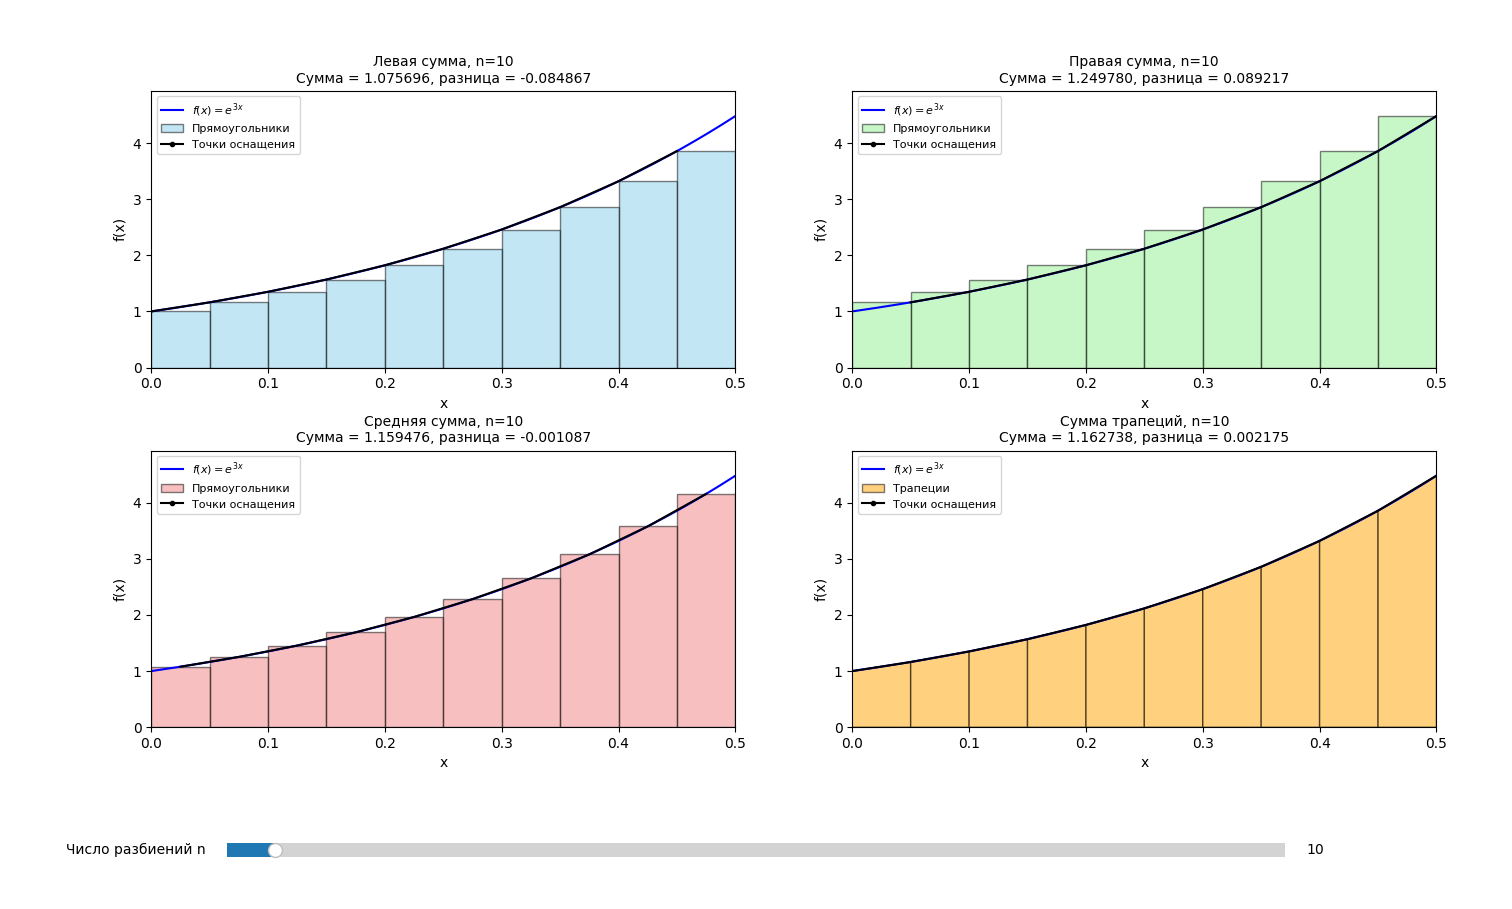
\includegraphics[width=0.8\textwidth]{mis_1.png}
\end{center}
\end{figure}


\dots дальше Григорий

\section{\textbf{ Маятник.}}

\subsection{Малые колебания}

\subsubsection{Исследование теоретического изменения угла от практического}

Для эксперимента была использована нить, длинной $L = 0.94 \text{ м}$. В таком случае, теоретическая частота $\omega = \sqrt{\dfrac{g}{L}} =  \sqrt{\dfrac{9.82}{0.94}} \approx 3.23 \text{ } c^{-1}$

Тогда, теоретическая зависимость угла от времени: $\theta = \theta_0\cos{(\omega t)}$

Начальные углы в каждой серии: 


\begin{table}[H]
    \centering
    \begin{tabular}{|p{2cm}|p{2cm}|p{2cm}|p{2.5cm}|p{2.5cm}|p{2.5cm}|}
        \hline 
        1 серия (малые углы) & 2 серия (малые углы) & 3 серия (малые углы) & 
        1 серия (большие углы) & 2 серия (большие углы) & 3 серия (большие углы) \\ 
        \hline 
        $\theta_0 = \ang{14.61}$ & $\theta_0 = \ang{6.22}$ & $\theta_0 = \ang{13.69}$ & 
        $\theta_0 = \ang{54.72}$ & $\theta_0 = \ang{55.00}$ & $\theta_0 = \ang{43.20}$ \\ 
        \hline
    \end{tabular}
    \caption{Начальные углы}
    \label{tab:value}
\end{table}

\begin{figure}[H]
    \begin{center}
    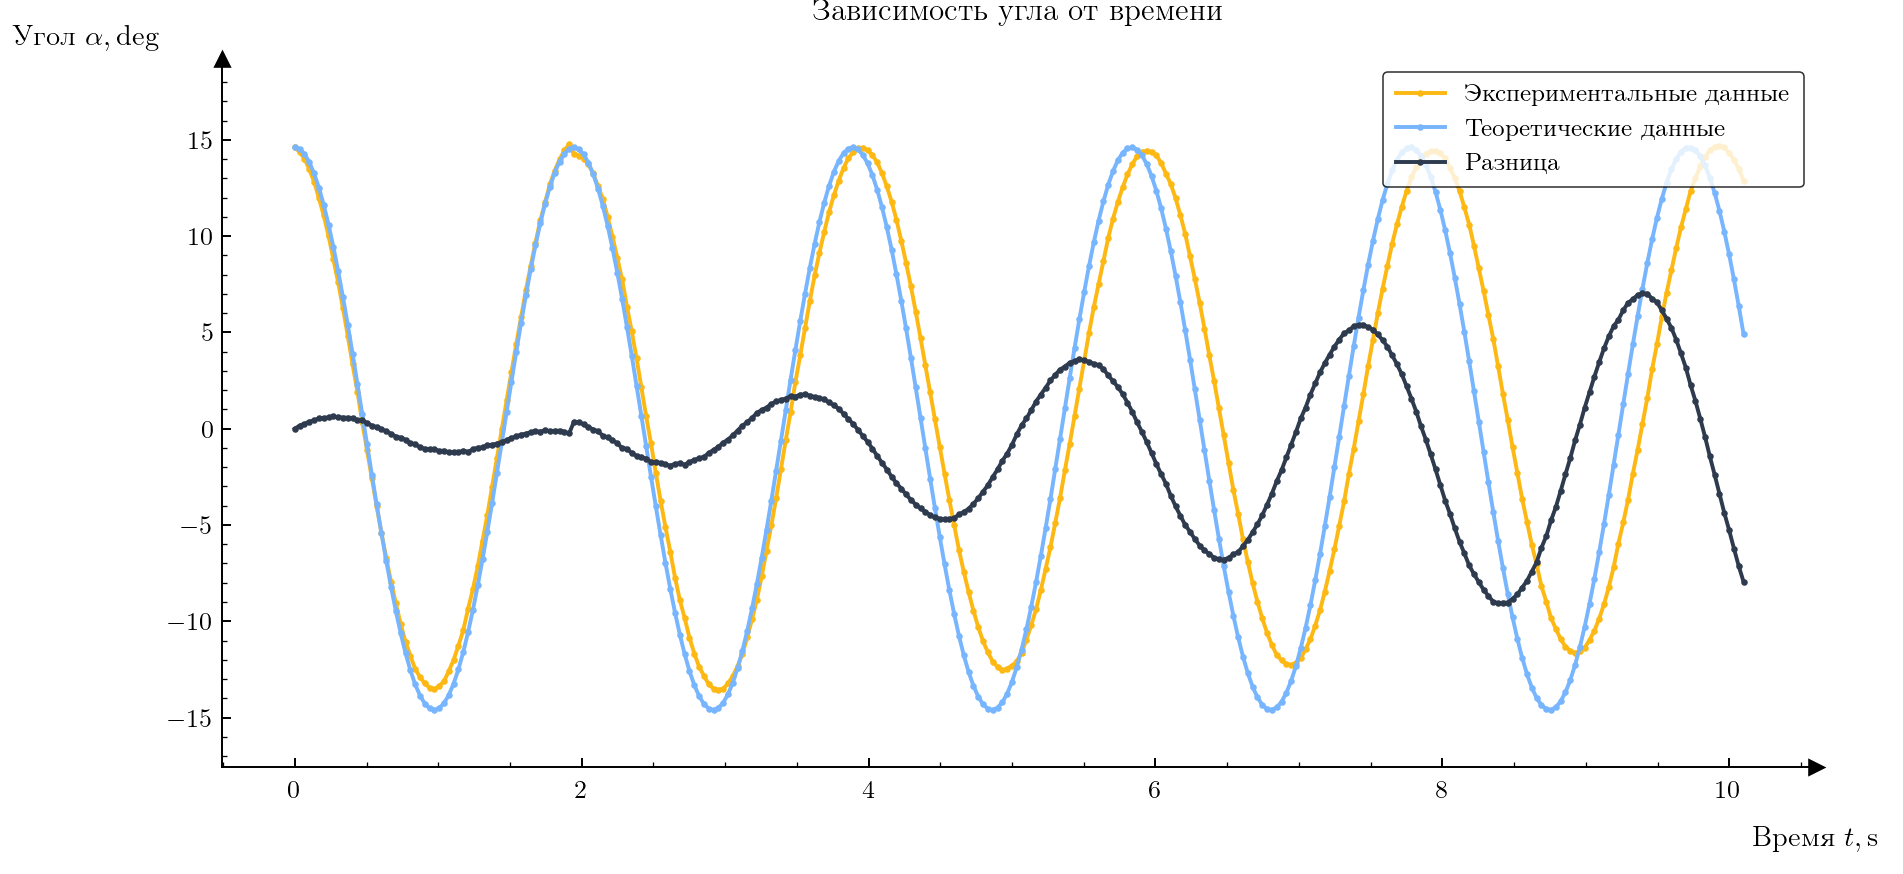
\includegraphics[width=1.11\textwidth]{1.png}
    \caption{1 серия}
\end{center}
\end{figure}
\begin{figure}[H]
    \begin{center}
    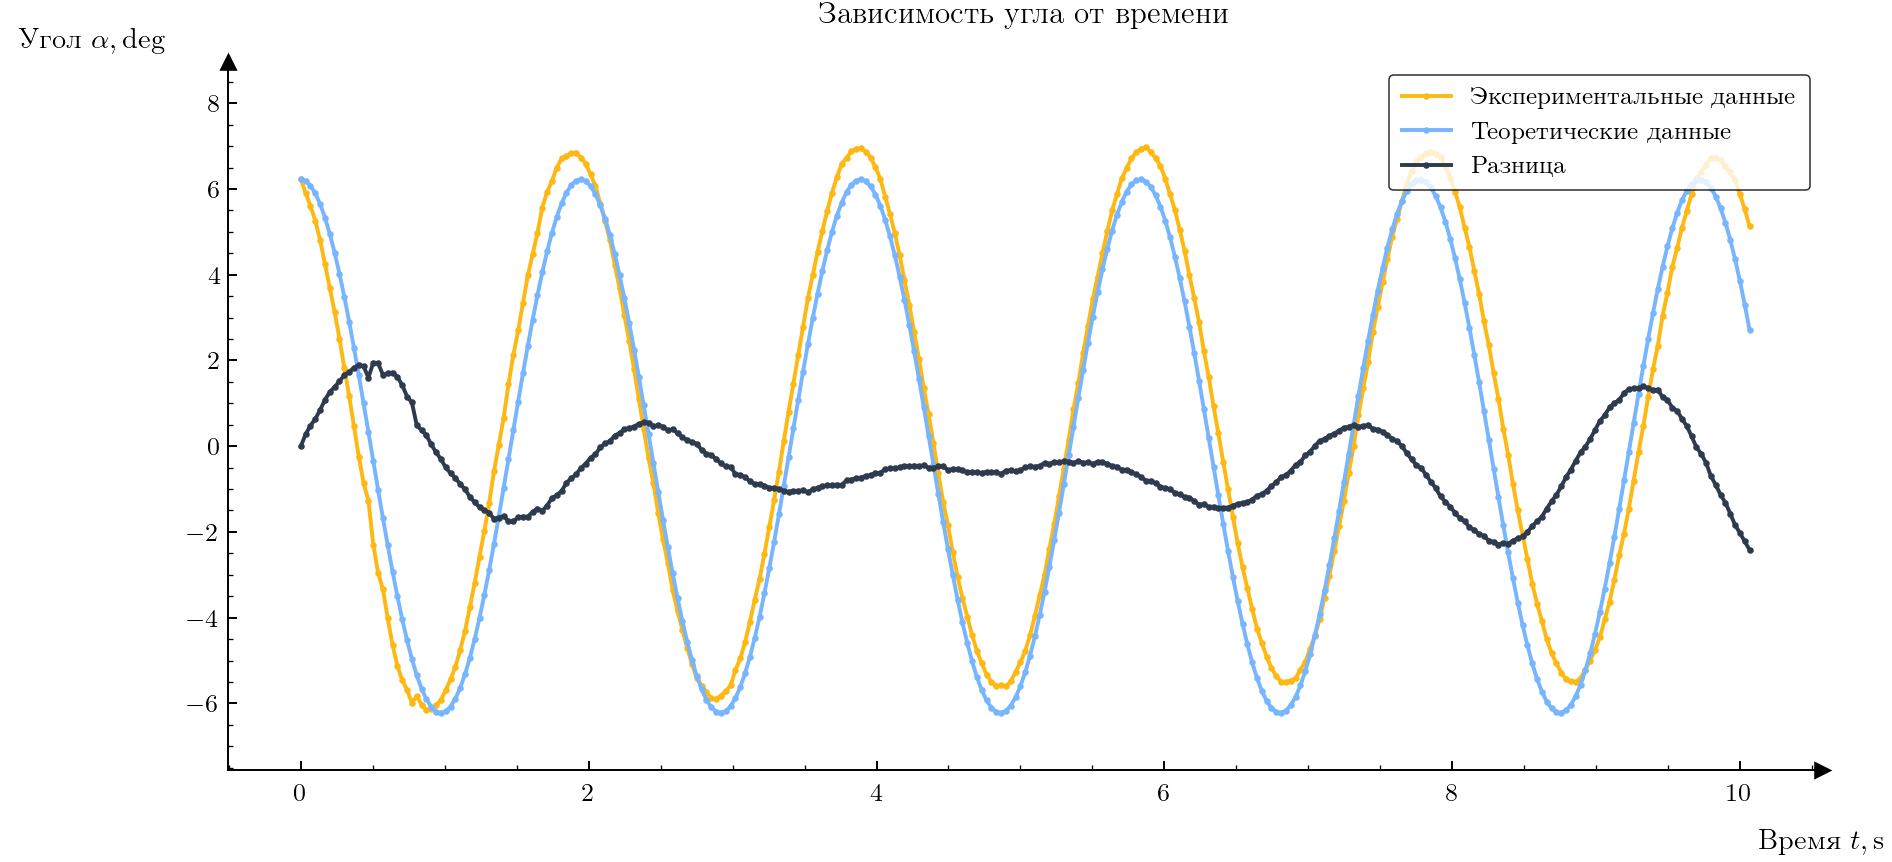
\includegraphics[width=1.11\textwidth]{2.png}
    \caption{2 серия}
\end{center}
\end{figure}
\begin{figure}[H]
    \begin{center}
    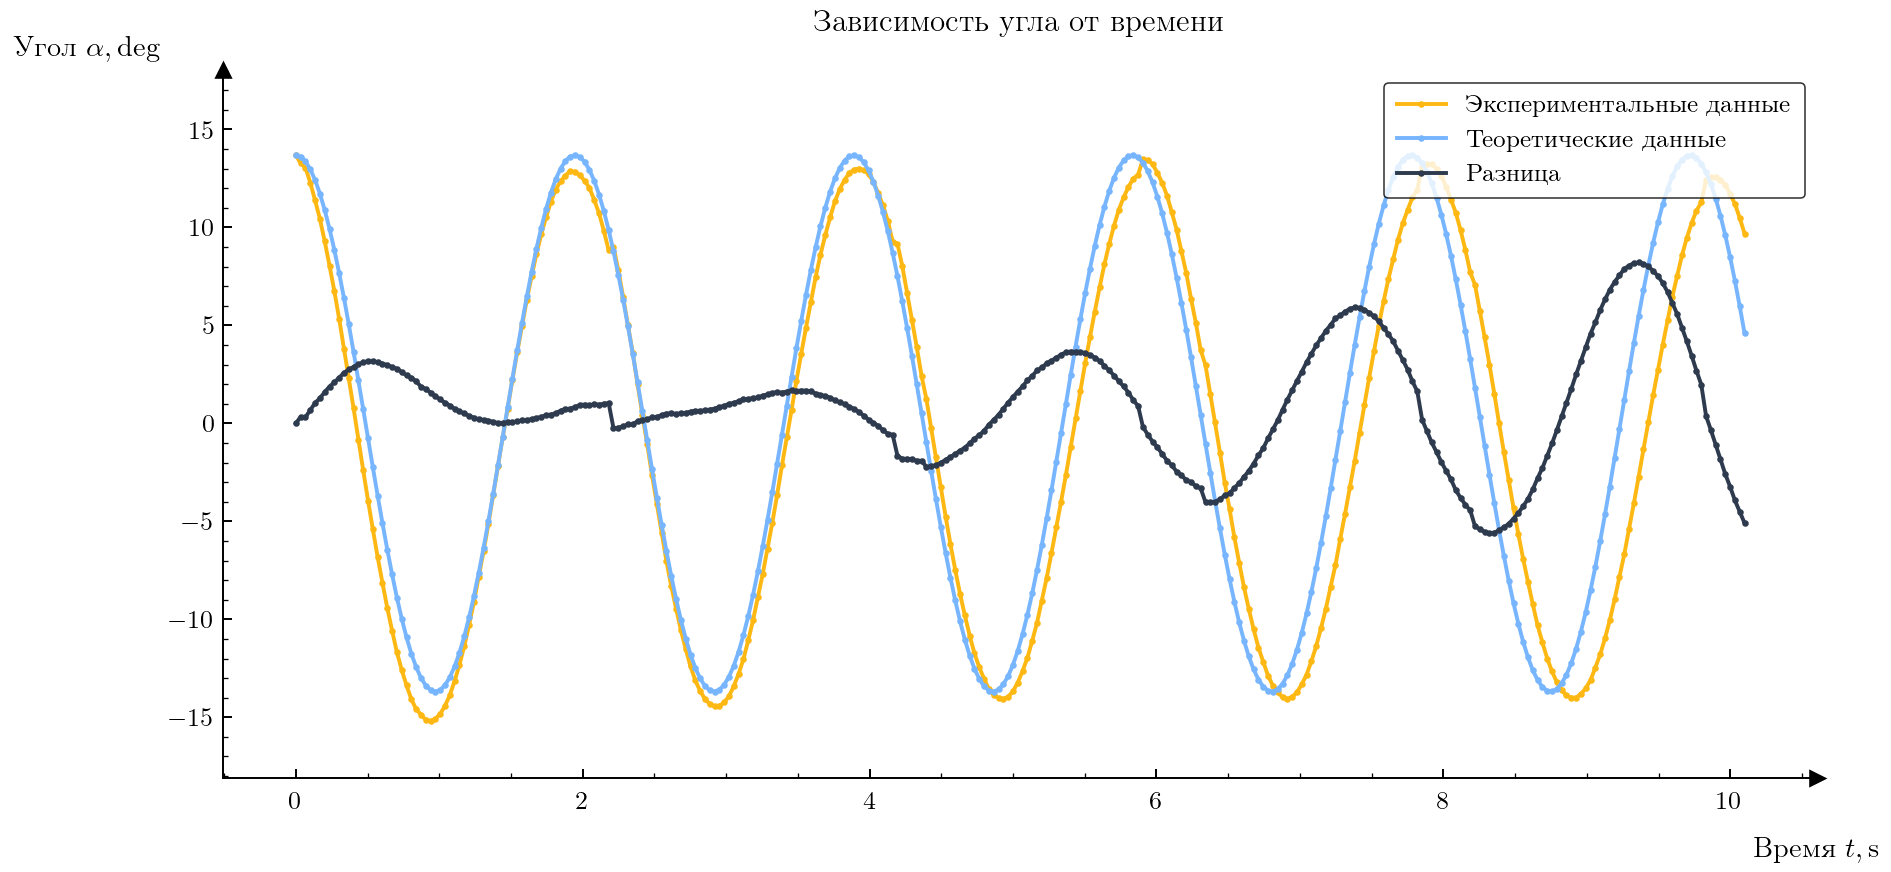
\includegraphics[width=1.11\textwidth]{3.png}
    \caption{3 серия}
\end{center}
\end{figure}

\subsubsection{Исследование изменения теоретического периода от практического}

Теоретически, период колебаний будет рассчитываться как $T = 2\pi\sqrt{\dfrac{l}{g}} = 1.94 \text{ с}$

Для серий эти периоды были равны (вычисляем как время 5 колебаний деленное на 5):

$T_1 \approx 2.10 \text{ с}$
$T_2 \approx 2.19 \text{ с}$
$T_3 \approx 2.01 \text{ с}$

\subsubsection{Объяснение перехода в (3)}

$\dot\theta = \pm\omega\sqrt{\theta_0^2-\theta^2}
\\
\dfrac{\dd\theta}{\dd t} = \pm\omega\sqrt{\theta_0^2-\theta^2}
\\
\dfrac{\dd\theta}{\sqrt{\theta_0^2-\theta^2}} = \pm\omega\dd t
\\
\int\limits_{\theta_0}^{\theta}\dfrac{\dd\theta}{\sqrt{\theta_0^2-\theta^2}} = \left.\arcsin{\dfrac{\theta}{\theta_0}} \right|_{\theta=\theta_0}^{\theta}=\arcsin{\dfrac{\theta}{\theta_0}} - \arcsin{\dfrac{\theta_0}{\theta_0}} = \arcsin{\dfrac{\theta}{\theta_0}} - \dfrac{\pi}{2}
\\
\int\limits_{0}^{t}\pm\omega\dd t = \pm\omega t \Rightarrow \dfrac{\theta}{\theta_0} = \sin{\left(\pm\omega t + \dfrac{\pi}{2}\right)} = \cos{(\omega t)} \text{ Ч.Т.Д.}
$
\subsubsection{Оценка погрешностей}

У нас имеется три серии, в который теоретически период должен быть одинаковый. Среднее значение практического периода колебания:

$\overline{T} = \dfrac{\sum T}{3} = 2.10 \text{ c}$

$\Delta t = \sqrt{t_{0.9;3}^2\dfrac{\sum(T_i-\overline{T})^2}{6}+\Delta t_{\text{пр}}^2} = 0.18 \text{ c}$

$\varepsilon_t = 8.6 \text{ \%}$

Тогда, значение $T$ с доверительным интервалом:

$T = 2.10\pm 0.18 \text{ c}$

Выводы: Теоретическое значение (1,94 с) не лежит в доверительном интервале полученного практически значения. Данное отличие может быть обусловлено наличием вязкого трения, т к при наличии такого трения уменьшается частота колебаний $\Rightarrow$ увеличивается период колебаний. Кроме того, не все колебания получились "идеально" малыми - двух из трех экспериментах угол чуть больше $\ang{10}$. 

Анализируя графики различия теоретического изменения угла от практически полученного можно наблюдать, что чем дольше идет наблюдение, тем больше погрешность. Если вначале это может быть связано с приближениями мат модели, то в конце большее влияние на погрешность поведения угла оказывает как раз различие в периоде.

\subsection{Нелинейные колебания}

\subsubsection{Исследование теоретического периода от практического}

Используя значения начальных углов в таблице, найдем теоретическое значение периода колебания (вычисляем инетеграл по сумме средних прямоугольников)
\\
$
T_1=2.02  \text{ с}
\\
T_2=2.02\text{ с}
\\
T_3=2.01\text{ с}
$

%Погрешность:
% \\
% $
% f'(x) = \dfrac{\cos\left(x\right)\,\sin\left(x\right)}{\left({\cos^{2}\left(x\right)-\cos^{2}\left(\theta_0\right)}\right)^{\frac{3}{2}}}$ -- на интервале $[0;1)$ монотонно растет $\Rightarrow$ $\max{\abs{f'{(x)}}} = f'(\theta_0)$
% \\
% $
% f'(0.96) = 
% $



Графики зависимости практического изменения угла от времени:

\begin{figure}[H]
    \begin{center}
    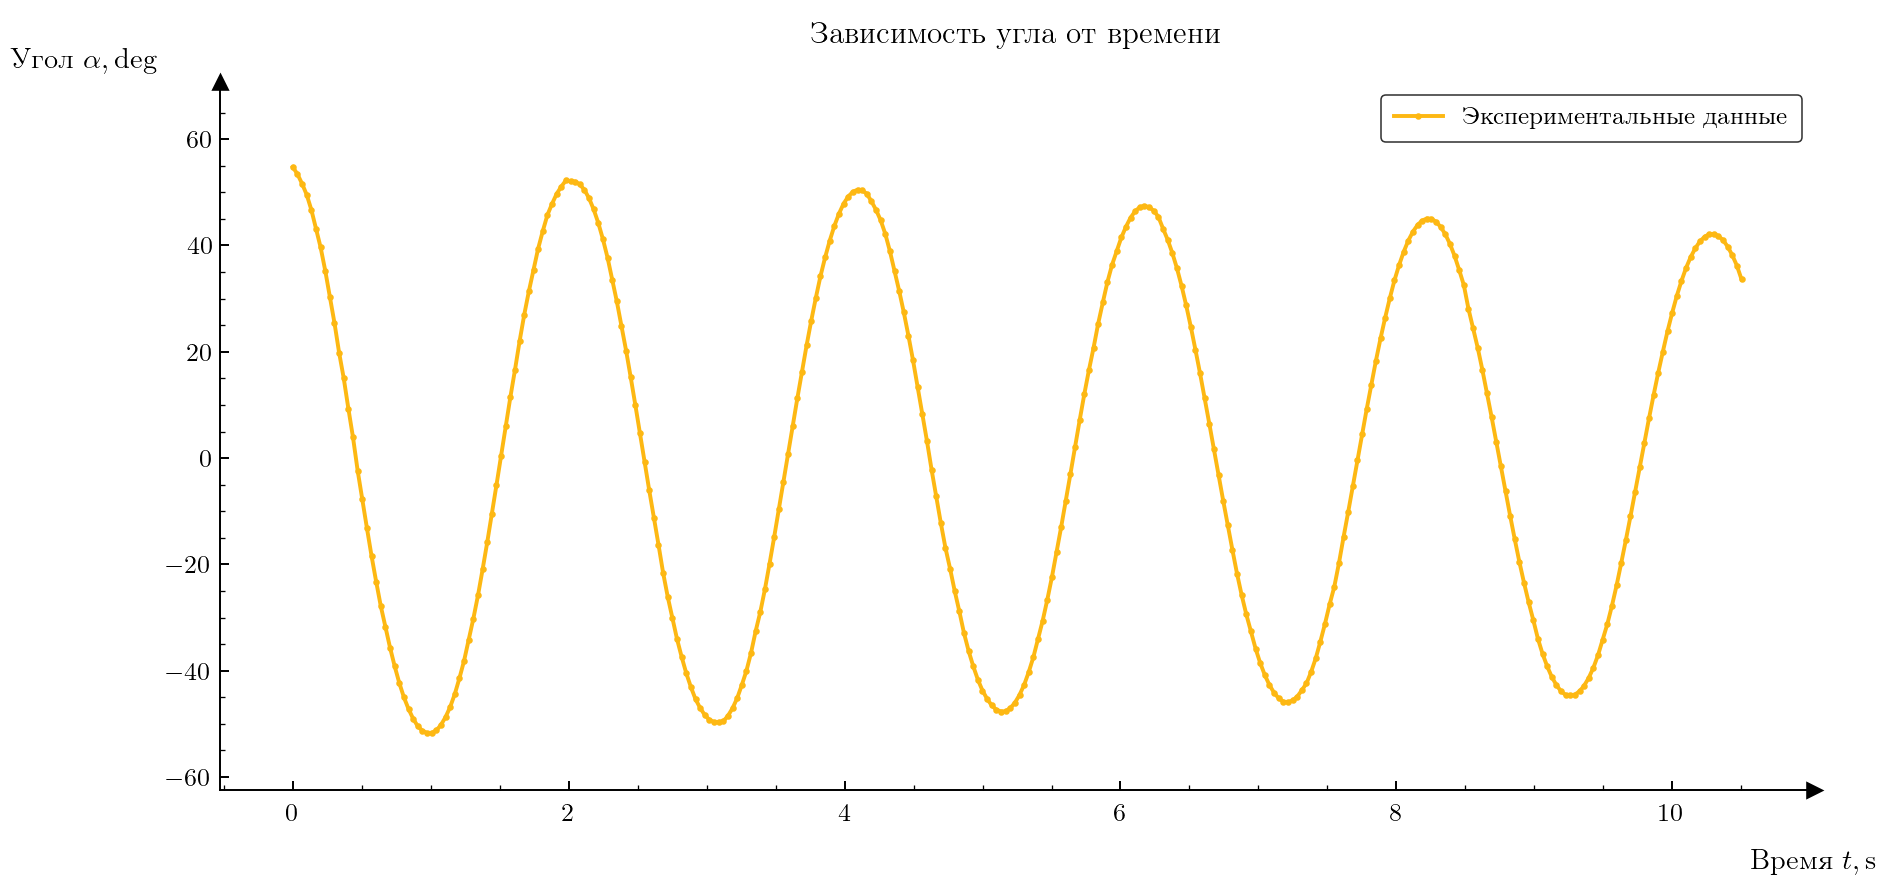
\includegraphics[width=0.8\textwidth]{4.png}
    \caption{$\theta_0 = \ang{54.72}$}
\end{center}
\end{figure}
\begin{figure}[H]
    \begin{center}
    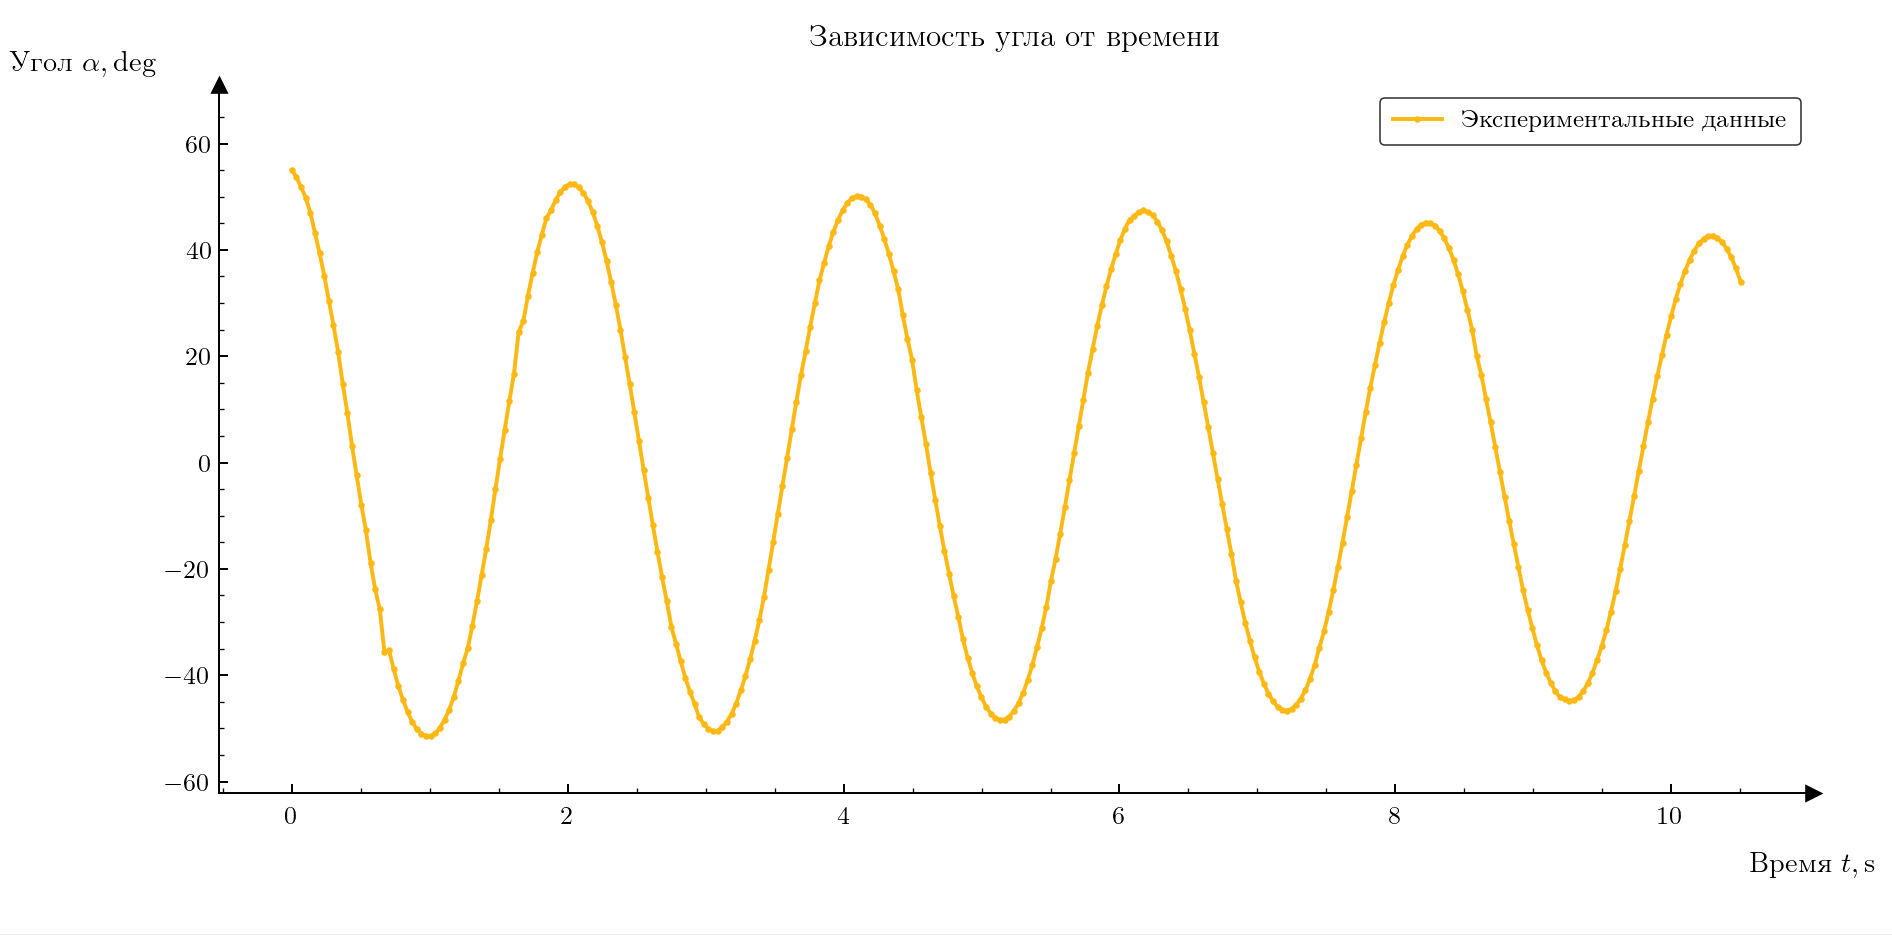
\includegraphics[width=0.8\textwidth]{5.png}
    \caption{$\theta_0 = \ang{55.00}$}
\end{center}
\end{figure}
\begin{figure}[H]
    \begin{center}
    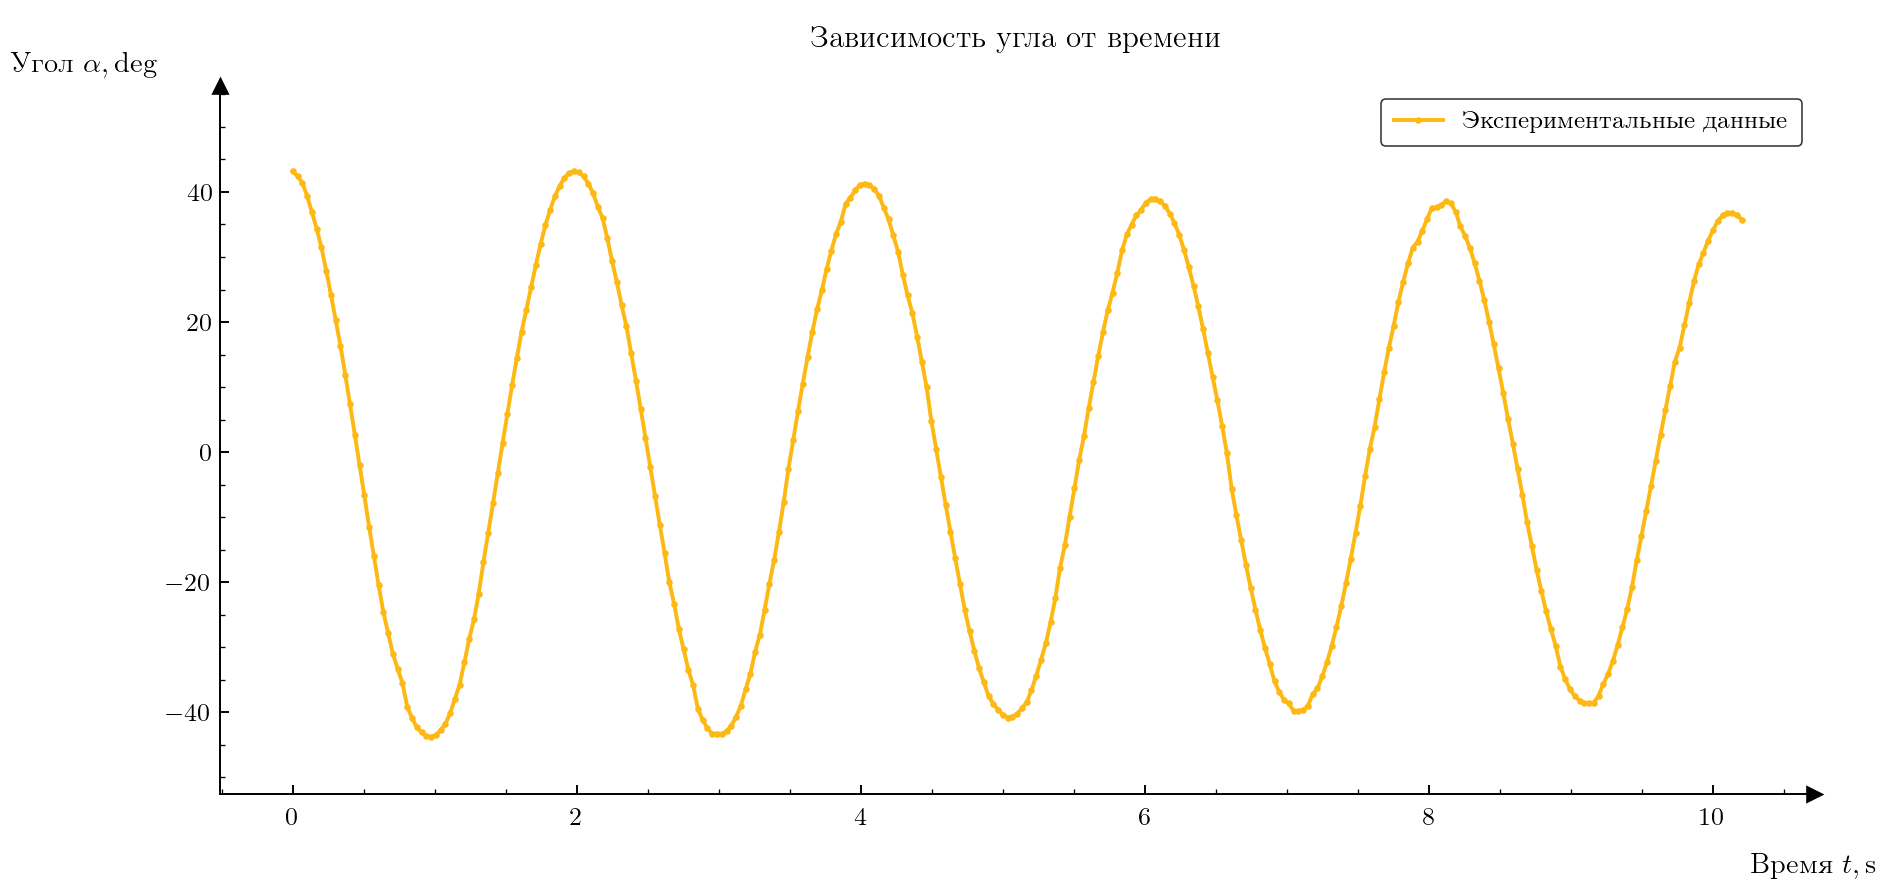
\includegraphics[width=0.8\textwidth]{6.png}
    \caption{$\theta_0 = \ang{43.20}$}
\end{center}
\end{figure}



Практически полученное значение периода колебаний от времени:
\\
$T_{1_{\text{прак}}} = 2.06 \text{ с}$
\\
$T_{2_{\text{прак}}} = 2.06 \text{ с}$
\\
$T_{3_{\text{прак}}} = 2.02 \text{ с}$

Таким образом, отличие теоретического периода от практического:
\\
$
\Delta_1 = 0.04\text{ с}
\\
\Delta_2 = 0.04\text{ с}
\\
\Delta_3 = 0.01\text{ с}
$

\subsubsection{Доказательство формулы (6)}


\begin{equation}
\cos\theta - \cos\theta_0 = 2\sin^2\left(\frac{\theta_0}{2}\right) - 2\sin^2\left(\frac{\theta}{2}\right) = 2k^2 - 2\sin^2\left(\frac{\theta}{2}\right)
\label{eq:trig_identity}
\end{equation}
где введено обозначение $k \equiv \sin\left(\frac{\theta_0}{2}\right)$.


Введём новую переменную $u$ через соотношение:
\begin{equation}
\sin u = \frac{\sin\left(\frac{\theta}{2}\right)}{k}
\label{eq:substitution}
\end{equation}


Продифференцируем подстановку:
\begin{equation}
\cos u \dd{u} = \frac{\cos\left(\frac{\theta}{2}\right)}{2k} \dd{\theta}
\end{equation}

\begin{equation}
\dd{\theta} = \frac{2k \cos u}{\cos\left(\frac{\theta}{2}\right)} \dd{u}
\end{equation}
Учитывая, что $\cos\left(\frac{\theta}{2}\right) = \sqrt{1 - k^2\sin^2 u}$, получаем:
\begin{equation}
\dd{\theta} = \frac{2k \cos u}{\sqrt{1 - k^2\sin^2 u}} \dd{u}
\label{eq:differential}
\end{equation}


Используя \eqref{eq:trig_identity}, выразим знаменатель:
\begin{equation}
\sqrt{\cos\theta - \cos\theta_0} = \sqrt{2}\sqrt{k^2 - \sin^2\left(\frac{\theta}{2}\right)} = \sqrt{2}k\sqrt{1 - \sin^2 u} = \sqrt{2}k\cos u
\end{equation}



\begin{equation}
\int \frac{\dd{\theta}}{\sqrt{\cos\theta - \cos\theta_0}} = \int \frac{1}{\sqrt{2}k\cos u} \cdot \frac{2k\cos u}{\sqrt{1 - k^2\sin^2 u}} \dd{u} = \sqrt{2} \int \frac{\dd{u}}{\sqrt{1 - k^2\sin^2 u}}
\end{equation}


\begin{itemize}
\item При $\theta = 0$: $\sin u = 0 \Rightarrow u = 0$
\item При $\theta = \theta_0$: $\sin u = 1 \Rightarrow u = \frac{\pi}{2}$
\end{itemize}

Итоговое преобразование
\begin{equation}
\int\limits_0^{\theta_0} \frac{\dd{\theta}}{\sqrt{\cos\theta - \cos\theta_0}} = \sqrt{2} \int\limits_0^{\pi/2} \frac{\dd{u}}{\sqrt{1 - k^2\sin^2 u}} = \sqrt{2} F\left(\frac{\pi}{2}, k\right)
\label{eq:result}
\end{equation}
где $F(\varphi,k)$ -- неполный эллиптический интеграл первого рода.


\subsubsection{Вычисление эллиптического интеграла}

\[
K(k) = \int\limits_0^{\pi/2} \frac{du}{\sqrt{1 - k^2 \sin^2 u}} 
      = \frac{\pi}{2} \sum_{n=0}^\infty \left( \frac{(2n-1)!!}{(2n)!!} k^n \right)^2,
      \quad (-1)!! = 1.
\]

\[
K(\sin{0.96}) = \int\limits_0^{\pi/2} \frac{du}{\sqrt{1 - k^2 \sin^2 u}} 
      = \frac{\pi}{2} \left(\left( \frac{(-1)!!}{(0)!!}\cdot \sin^0(0.96) \right)^2 +\left( \frac{(2-1)!!}{(2)!!}\cdot \sin(0.96) \right)^2\right) = 1.83 \text{, n  = 1}
\]
\[
K(\sin{0.96}) = \int\limits_0^{\pi/2} \frac{du}{\sqrt{1 - k^2 \sin^2 u}} = 1.93 \text{, n  = 2}
\]
\[
K(\sin{0.96}) = \int\limits_0^{\pi/2} \frac{du}{\sqrt{1 - k^2 \sin^2 u}} = 1.98 \text{, n  = 3}
\]


\[
K(\sin{0.75}) = \int\limits_0^{\pi/2} \frac{du}{\sqrt{1 - k^2 \sin^2 u}} 
      = \frac{\pi}{2} \left(\left( \frac{(-1)!!}{(0)!!}\cdot \sin^0(0.96) \right)^2 +\left( \frac{(2-1)!!}{(2)!!}\cdot \sin(0.96) \right)^2\right) = 1.75 \text{, n  = 1}
\]
\[
K(\sin{0.75}) = \int\limits_0^{\pi/2} \frac{du}{\sqrt{1 - k^2 \sin^2 u}} = 1.80 \text{, n  = 2}
\]
\[
K(\sin{0.75}) = \int\limits_0^{\pi/2} \frac{du}{\sqrt{1 - k^2 \sin^2 u}} = 1.81 \text{, n  = 3}
\]

Можно сделать вывод, что при использовании трех слагаемых сумма стремительно приближается к вычисленному численно значению интеграла (это очень круто).

\subsubsection{Итоговые погрешности}

\[
 \left( \frac{1}{\sqrt{\cos \theta - \cos \theta_0}} \right)'' = \frac{3 \sin^2 \theta}{4 (\cos \theta - \cos \theta_0)^{5/2}} + \frac{\cos \theta}{2 (\cos \theta - \cos \theta_0)^{3/2}}
\]

Очевидно, что максимум значения этой производной при $\theta\rightarrow\theta_0$. . Тогда, для:
\\
$\theta_0 = 0.75$
\\
Чтобы избавиться от особенностей, делаем замену:
\\
$t = \sqrt{0.75-\theta}$. Тогда исходный интеграл и его вторая производная принимают следующий вид:
\\
\[
\left(\frac{t }{\sqrt{\cos(0.75 - t^2) - \cos 0.75}}\right)'' = \]
\[
f''(t) = \frac{-2u \cdot (2t \sin \phi) - t \cdot (2 \sin \phi + 4t^2 \cos \phi) \cdot u + \frac{3}{2} t \cdot (2t \sin \phi)^2}{u^{5/2}}
\]

где:
\begin{itemize}
    \item \( u = \cos(0.75 - t^2) - \cos 0.75 \),
    \item \( \phi = 0.75 - t^2 \).
\end{itemize}

В этом случае, погрешность вычисленного интеграла $\abs{R_n}\approx3\cdot10^{-7}$

Аналогично делаем для $\theta\approx0.96$. В этом случае замена: $t = \sqrt{0.75-\theta}$. В этом случае, погрешность составит $\abs{R_n} \approx 9\cdot10^{-7}$
\end{document}
